\chapter{Effect of Transport on Soot Evolution\label{ch:transport}}

The lifetime of soot is governed by the balance between growth and oxidation. Nucleation from collisions between PAH dimers~\cite{blanquart2009,schuetz2002,frenklach1991,wang2011}, condensation of PAH dimers on existing soot particles~\cite{blanquart2009,hmom2009}, and surface growth through the HACA surface reaction mechanism~\cite{frenklach1985,frenklach1991} are processes that increase soot mass by extracting species from the gas-phase. Conversely, oxidation by \ce{OH} and \ce{O2} removes carbon from particles~\cite{stanmore2001,neoh1981,kazakov1995} and can lead to their fragmentation and destruction~\cite{neoh1984,mueller2011}. Clearly, the dynamics of soot are governed by species with a broad range of chemical timescales and molecular weights. Therefore, accurately capturing interactions with gas-phase species is crucial when developing predictive models for soot evolution.

In \cref{ch:lesmodels}, the modeling foundation for LES was established. In particular, the classical nonpremixed flamelet equations for species and temperature~\cite{peters1984} were presented in \cref{sec:lesmodels:combust:flamelet} with modifications accounting for the formation of soot and radiative thermal losses. These equations were derived under the assumption that the species' effective Lewis numbers are unity. This assumption is based on the reasoning that turbulence mixes indiscriminately at sufficiently large Reynolds number~\cite{pitsch19981057}.

%% These equations were derived by transforming the physical space coordinate system of \cref{eq:lesmodels:combust:flamelet:consy,eq:lesmodels:combust:flamelet:const} to a mixture-fraction-based coordinate system. The latter conservation equations used Fick's law to evaluate the diffusion velocity, so all species were assumed to have the same constant diffusion coefficient $D$. A further simplication was made by selecting $D$ such that the species' effective Lewis numbers are unity, for it is often assumed that turbulence mixes all species indiscriminately at sufficiently high Reynolds numbers~\cite{pitsch19981057}.

However, DNS studies~\cite{bisetti2012,attili2014} have suggested that this assumption may be inappropriate for PAH, which are very sensitive to the local scalar dissipation rate due to their slow formation chemistry. These species are confined to spatially intermittent regions of low scalar dissipation rate that are on the order of the Kolmogorov scale or smaller~\cite{vaishnavi2008}. At such scales, transport is solely dictated by molecular diffusion. Therefore, a method to identify such strain-sensitive species and properly account for their interactions with soot is desired. The development of a model that addresses these points is the focus of this chapter.

%% Summary: Main point of chapter is to show that existing transport models do not properly account for the presence of soot. As a result, a strain sensitive transport model is developed.

%% Include a brief introduction explaining why accurately capturing the transport of gas-phase species is important for developing predictive models for soot evolution in LES (growth and oxixidation processes).

% include other files for sections of this chapter. These use the 'input' command since each section within a chapter should not start a new page.
% If you want to swap the order of sections, it is as simple as reversing the order you include them. 
\section{Overview of Gas-Phase Species Transport}
\label{sec:transport:overview}

%% \subsection{Equal Effective Diffusivities}
%% \label{sec:transport:overview:le1}

%% Summary of equal effective diffusivities approach.


\subsection{Considerations for PAH}
\label{sec:transport:overview:pah}

The nonpremixed flamelet equations for species and temperature were derived in \cref{sec:lesmodels:combust:flamelet} while assuming that species mass fraction and temperature gradients parallel to the mixture fraction gradient dominate and that the species' effective Lewis numbers are unity. The theory behind the latter assumption states that, at sufficiently large Reynolds number, the smallest scales of turbulence (Kolmogorov scales) penetrate the fuel-oxidizer mixing zone of the nonpremixed flame~\cite{peters1984}. Consequently, turbulent mixing dominates molecular mixing within this region, and all species are transported with unity effective Lewis numbers. This line of reasoning implicitly assumes that the species' length scales are comparable to the fuel-oxidizer mixing length scale, which is certainly true for the major combustion products such as \ce{CO}, \ce{CO2}, \ce{H2}, and \ce{H2O}.

However, the DNS studies of Bisetti \etal~\cite{bisetti2012} and Attili \etal~\cite{attili2014} suggest otherwise for PAH, which play an integral role in soot nucleation and condensation. In \cref{fig:transport:overview:pah:unsteadypah}, the mass fractions of acetylene and naphthalene from the DNS are compared to the values from the one-dimensional steady flamelet equation solutions under the same set of conditions (unity Lewis number, no Soret and Dufour effects, same reduced chemical mechanism, etc.). It is evident that, as the scalar dissipation rate is increased, the mass fraction of acetylene falls from $2 \times 10^{-2}$ to $1 \times 10^{-2}$ while the mass fraction of naphthalene decreases two orders of magnitude from $10^{-4}$ to $10^{-6}$. Naphthalene is clearly more sensitive to the local value of scalar dissipation rate, which is a result of its slow formation chemistry. An elevated local scalar dissipation rate minimizes the time for larger hydrocarbon species to collide and successfully react, so the presence of PAH is restricted to a limited range of low scalar dissipation rates.

\begin{figure}[ht]
  \centering
  \begin{subfigure}[b]{0.375\linewidth}
    \centering
    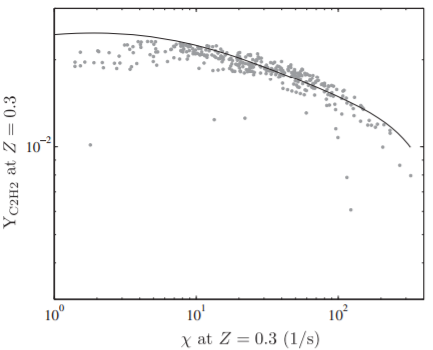
\includegraphics[width=\linewidth]{ch-transport/figures/dns-YC2H2vschi}
  \end{subfigure}%%
  \begin{subfigure}[b]{0.375\linewidth}
    \centering
    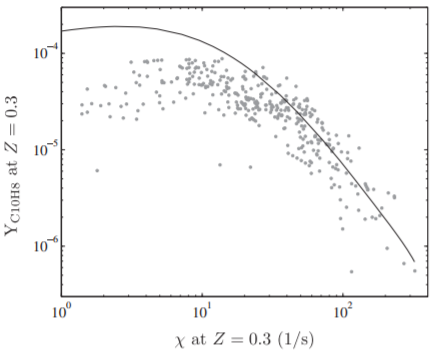
\includegraphics[width=\linewidth]{ch-transport/figures/dns-YC10H8vschi}
  \end{subfigure}
  \caption[Effects of Scalar Dissipation Rate on \texorpdfstring{$Y_{\ce{C2H2}}$}{YC2H2} and \texorpdfstring{$Y_{\ce{C10H8}}$}{YC10H8}]{Mass fraction of acetylene and naphthalene as a function of scalar dissipation rate, reproduced from Bisetti \etal~\cite{bisetti2012}. Samples are taken at $t = 5$ ms and $Z = 0.3$ from the same DNS conditions of \cref{fig:subfilter:zussp:chisensitivity}. Solid lines are the steady flamelet solutions.}
  \label{fig:transport:overview:pah:unsteadypah}
\end{figure} 

Additionally, the steady flamelet solutions tend to capture the overall decreasing trend of the DNS samples for both acetylene and naphthalene, although significant scatter about the steady solution is present for naphthalene. This deviation is caused by naphthalene's inability to adjust to the rapidly changing turbulent flow field and corresponding scalar dissipation rate as a result of its slow chemistry. PAH larger than naphthalene are anticipated to possess similar characteristics. On the other hand, the chemistry of acetylene is much faster, allowing it to persist in regions of larger scalar dissipation rate.
%The scatter is more significant at lower values of scalar dissipation rate, which is due to unsteady flamelet effects~\cite{turbulentcombustion,bisetti2012}.

As a result of the above phenomena, PAH are confined to spatially intermittent regions of low scalar dissipation rate, which are visible in \cref{fig:subfilter:zussp:chisensitivity} for naphthalene. These regions are on the order of the Kolmogorov scale or smaller~\cite{vaishnavi2008}, where transport is solely dictated by molecular diffusion. Therefore, it is worthwhile to examine the effects of molecular transport on the evolution of these soot precursors. Flamelet models that incorporate differential diffusion are presented in the following subsection.


\subsection{Molecular Transport}
\label{sec:transport:overview:lei}

Pitsch and Peters~\cite{pitsch1998} previously derived a set of one-dimensional nonpremixed flamelet equations for flat flames accounting for differential diffusion effects. Assuming variable, nonunity species Lewis numbers and a unity mixture fraction Lewis number, the species equation is given by
\begin{equation}\label{eq:transport:overview:lei:flamelety}
  \rho\pder[Y_k]{\tau} = \frac{\rho\chi}{2 Le_k}\sder[Y_k]{Z} + \dot{m}_k + \frac{\rho\chi}{2 Le_k}\frac{Y_k}{W}\sder[W]{Z} + V_k^{DD},
\end{equation}
where the species Lewis numbers $Le_k = \lambda/c_p\rho D_k$ represent the ratio of thermal to mass diffusivities.
%, $D_k = (1 - Y_k)/\sum\limits_{k \neq l} (X_k/D_{k,l})$ is the mixture-averaged diffusivity for species $k$, and $\chi = 2D_Z(\partial Z/\partial x_j)^2$ is the scalar dissipation rate. The diffusion velocities are expressed by the Curtiss-Hirschfelder approximation~\cite{curtiss1949} with a velocity correction to enforce mass conservation. These remaining molecular transport correction terms are lumped into $V_k^{DD}$ and are outlined in Pitsch and Peters~\cite{pitsch1998}. Similarly, the one-dimensional, adiabatic temperature equation is given by
\begin{equation}\label{eq:transport:overview:lei:flamelett}
  \rho c_p \pder[T]{\tau} = \frac{\rho c_p \chi}{2}\sder[T]{Z} + \frac{\rho\chi}{2}\pder[c_p]{Z}\pder[T]{Z} - \sum\limits_{k} h_k\dot{m}_k + \sum\limits_{k} \frac{\rho\chi}{2 Le_k}\left( \pder[Y_k]{Z} + \frac{Y_k}{W}\pder[W]{Z} \right)(c_p - c_{p,k})\pder[T]{Z},
\end{equation}
where $W$ is the molecular weight of the mixture and pressure variations have been neglected. Note that \cref{eq:transport:overview:lei:flamelety,eq:transport:overview:lei:flamelett} have been derived while assuming that the nonpremixed flame is one-dimensional in physical space \textit{a priori}. This assumption is convenient in the limit of a thin, one-dimensional flat flame, but is not appropriate for thick or curved flames. Recently, Xuan \etal~\cite{xuan2014} re-derived the flamelet equations accounting for differential diffusion while assuming that the nonpremixed flame is one-dimensional in mixture fraction space \textit{a posteriori} in order to capture curvature effects. Although the latter formulation will not be used in the remainder of this work, curvature effects can significantly affect transport in mixture fraction space, and analysis of curvature effects on PAH evolution in turbulent nonpremixed combustion is a suggestion for future work.

Attili \etal~\cite{attili2016} conducted two three-dimensional direct numerical simulations of the same configuration as previously described in \cref{sec:subfilter:dns}, with a modified domain size of $L_x \times L_y \times L_z = 105 \times 94 \times 47$ mm. A mixture-averaged transport approach was employed in one DNS, while the other modeled transport of gas-phase species with unity Lewis numbers. These two simulations were compared to analyze the influence of the diffusion model on the flame structure and soot formation. Their results at $t = 15$ ms, shown in \cref{fig:transport:overview:lei:a2vsz}, indicate that acetylene is unaffected by differential diffusion while naphthalene is strongly affected by the molecular transport model. The locations of the peaks for the latter species are the same for both transport models, but the magnitudes vary by more than a factor of two. These trends are consistent across all times in the DNS and suggest the importance of differential diffusion in predicting the yield of naphthalene and other larger PAH. Attili \etal~\cite{attili2016} noted that the mixture-averaged approach lead to smaller amounts of diffusion (larger Lewis number) of naphthalene than the equal diffusivities approach. As a consequence, the naphthalene structures were found to be smaller and characterized by larger peaks. These ultimately affect the formation of soot due to the non-linearity of the soot source terms with respect to the concentration of PAH species.

\begin{figure}[htb]
  \centering
  \includegraphics[width=0.6\linewidth]{ch-transport/figures/DNSComparison-A2-C2H2}
  \caption[DNS Results with \texorpdfstring{$Le = 1$}{Le = 1} and \texorpdfstring{$Le \neq 1$}{Le != 1}, \texorpdfstring{$\langle Y_{\ce{C2H2}}|Z \rangle$}{<YC2H2|Z>} \& \texorpdfstring{$\langle Y_{\text{A2}}|Z \rangle$}{<YA2|Z>} vs. \texorpdfstring{$Z$}{Z}]{Means of acetylene (\ce{C2H2}) and naphthalene (\ce{A2}) mass fraction conditioned on mixture fraction at $t = 15$ ms, reproduced from Attili \etal~\cite{attili2016}. The filled squares are transport with mixture-averaged diffusion, and the open circles are the $Le = 1$ case. The vertical black dashed line marks the location of stoichiometric mixture fraction $Z_{st} = 0.147$.}
  \label{fig:transport:overview:lei:a2vsz}
\end{figure}

On the other hand, it was also observed that the detailed transport model had a less significant influence on predictions of the temperature and the mass fractions of species that participate in the heat-releasing chemistry. In \cref{fig:transport:overview:lei:tvsz}, there is very little difference between the profiles from the two simulations for the temperature and hydroxyl mass fraction. The discrepancy between the transport models is larger for the hydrogen radical mass fraction profile (not shown), although this may be the result of an only moderate Reynolds number. Flamelet solutions with equal effective diffusivities track the unity Lewis number profiles from the DNS fairly well, unlike the solutions with detailed transport, which deviate from the DNS with the corresponding model.

It is clear that there is a simultaneous presence of transport by molecular diffusion for species that are confined to regions on the order of the Kolmogorov scale or smaller and transport by turbulent eddies for species that participate in faster chemistry. A model for gas-phase species transport that attempts to account for unity and nonunity Lewis numbers is presented in the upcoming subsection.

\begin{figure}[htb]
  \centering
  \includegraphics[width=\linewidth]{ch-transport/figures/DNSComparison-T-OH}
  \caption[DNS Results with \texorpdfstring{$Le = 1$}{Le = 1} and \texorpdfstring{$Le \neq 1$}{Le != 1}, \texorpdfstring{$\langle T|Z \rangle$}{<T|Z>}, and \texorpdfstring{$\langle Y_{\ce{OH}}|Z \rangle$}{<YOH|Z>} vs. \texorpdfstring{$Z$}{Z}]{Means of temperature and hydroxyl mass fraction conditioned on mixture fraction at $t = 15$ ms, reproduced from Attili \etal~\cite{attili2016}. The filled squares are transport with mixture-averaged diffusion, and the open circles are the $Le = 1$ case. One-dimensional nonpremixed flamelet solutions are indicated by the dashed lines (mixture-averaged) and solid lines ($Le = 1$). The vertical black dashed line is the same as in \cref{fig:transport:overview:lei:a2vsz}.}
  \label{fig:transport:overview:lei:tvsz}
\end{figure}


\subsection{Bimodal Transport}
\label{sec:transport:overview:bimodal}

% \Cref{eq:transport:overview:lei:flamelety,eq:transport:overview:lei:flamelett} have been observed to overpredict the amount of differential diffusion in the downstream region of a turbulent jet flame~\cite{pitsch2000}. This behavior has been explained by the decreased Reynolds number in that region, where a diminished scalar dissipation rate permits the smallest scales of turbulence to enter the broadened mixing zone.
The flamelet equations of \cref{sec:lesmodels:combust:flamelet} were derived for very high Reynolds number flows, where it is assumed that only turbulent transport is important. Conversely, \cref{eq:transport:overview:lei:flamelety,eq:transport:overview:lei:flamelett} were derived while assuming that only molecular transport matters, which is applicable to laminar flows. However, for a finite Reynolds number, the truth is in between. Recently, Wang~\cite{wang2016} introduced a Reynolds number dependence into the flamelet framework in order to address this point. To measure the degree of differential molecular diffusion, Wang defined a parameter
\begin{equation}\label{eq:transport:overview:bimodal:theta}
  \theta(r)= \frac{r}{1 + r},
\end{equation}
where $r$ is the ratio of the molecular diffusivity to the turbulent diffusivity and is inversely proportional to the Reynolds number. At the limit of an infinite Reynolds number, the influence of molecular diffusion vanishes as transport by turbulent eddies becomes dominant. In this limit, $r$ and $\theta(r)$ both approach zero. Conversely, when the Reynolds number approaches zero in the laminar limit, the effect of molecular diffusion is maximized, and $r$ tends to infinity. For this situation, $\theta(r)$ approaches unity.

Incorporation into \cref{eq:transport:overview:lei:flamelety,eq:transport:overview:lei:flamelett} is achieved by defining an effective Lewis number for species $k$:
\begin{equation}\label{eq:transport:overview:bimodal:lek}
  \hat{Le}_k = \frac{Le_k}{Le_k + \theta(r) \cdot (1 - Le_k)}.
\end{equation}
The form of this nonlinear dependence on $\theta$ was selected based on the analysis of a turbulent mixing layer~\cite{wang2016}. In the limit of infinite Reynolds number, $\theta = 0$ and $\hat{Le}_k = 1$ to model transport by turbulent diffusion. In the laminar limit, $\theta = 1$ and $\hat{Le}_k = Le_k$ to capture the effects of differential diffusion. %This effective Lewis number is not a physical property anymore, but it allows the aforementioned modes of transport to be modeled by simply replacing all instances of $Le_k$ in \cref{eq:transport:overview:lei:flamelety,eq:transport:overview:lei:flamelett}.

Despite its advancements of the flamelet framework, this model is still inappropriate for sooting flames. Wang's approach implicitly assumes that the length scales of all species are on the order of the thickness of the mixing zone, which varies with respect to the turbulent length scales as a function of Reynolds number. As the Reynolds number varies in a certain region, all species are governed by the mode of transport dictated by \cref{eq:transport:overview:bimodal:theta}. However, from \cref{sec:transport:overview:lei}, it is known that PAH are confined to regions that are on the order of the Kolmogorov scale or smaller due to their slow formation chemistry. At these scales, differential molecular diffusion overwhelms transport by turbulent eddies irrespective of the Reynolds number. Therefore, another model must be formulated to account for these properties of PAH and other species that are governed by slow kinetics. An approach that incorporates the idea of differential differential diffusion is introduced in \cref{sec:transport:ssta}.

\section{Strain-Sensitive Transport Approach}
\label{sec:transport:ssta}

\subsection{Model Development}
\label{sec:transport:ssta:framework}

Using the nonpremixed flamelet framework provided by \cref{eq:transport:overview:lei:flamelety,eq:transport:overview:lei:flamelett}, the proposed model applies molecular transport to particular species rather than to all species within regions of a certain Reynolds number. Selection of these species is through the strain-sensitivity parameter
\begin{equation}\label{eq:transport:ssta:framework:ssp}
  \zeta_k \equiv \frac{\rho\chi}{\dot{m}_k^{+}},
\end{equation}
where $\dot{m}_k^{+}$ is the chemical production rate of species $k$. When $\zeta_k > 1$, the rate of local mixing is greater than the formation chemistry rate (\textit{i.e.}, the chemistry is slow). Species $k$ is then identified as strain-sensitive and is confined to scales on the order of Kolmogorov or smaller, where molecular transport is dominant. Conversely, when $\zeta_k < 1$, the formation chemistry is fast, and the effective diffusivity of species $k$ is governed by the turbulent diffusivity. In this case, the length scales are now comparable to those of fuel-oxidizer mixing (such as for major species).

The strain-sensitivity parameter is shown for a selection of gas-phase species relevant to soot in \cref{fig:transport:ssta:framework:sspc7h16}. It is clear that $\zeta_{\text{A2}} > 1$ for any value of mixture fraction, indicating that differential diffusion for gas-phase naphthalene and larger PAH is important. Conversely, the strain-sensitivity parameters for acetylene, hydroxyl, and hydrogen are less than unity at slightly rich conditions, indicating that turbulent transport is dominant. Such a finding agrees with \cref{fig:transport:overview:lei:a2vsz,fig:transport:overview:lei:tvsz}, where differential diffusion is shown to be relevant for naphthalene but not for the other species. At this stage in model development, the minimum value of $\zeta_k$ is used to determine whether or not the species is strain-sensitive. This value provides the most conservative estimate for the species for which differential diffusion is important.

\begin{figure}[htb]
  \centering
  \includegraphics[width=0.43\linewidth]{ch-transport/figures/ZETAvsZ-C7H16-chi_st20}
  \caption[Strain-Sensitivity Parameter $\zeta_k$ for Various Species Within a \ce{C7H16}/\ce{N2} Mixture]{Strain-sensitivity parameter calculated from nonpremixed flamelet solutions for various species at $\chi_{st} = 20$ s$^{-1}$. The nitrogen-diluted, \textit{n}-heptane fuel mixture is the same as in \cref{fig:subfilter:zussp:chisensitivity}. The red line is for A2, the black line is for \ce{C2H2}, the blue line is for \ce{OH}, and the cyan line is for \ce{H}. The vertical black dashed line indicates the stoichiometric mixture fraction.}
  \label{fig:transport:ssta:framework:sspc7h16}
\end{figure}

A new definition of the effective species Lewis number $\check{Le}_k$ is required that depends on $\zeta_k$:
\begin{equation}\label{eq:transport:ssta:framework:lezetai}
  \check{Le}_k(\zeta_k) = \frac{Le_k}{Le_k + H(\min(\zeta_k) - 1)\cdot (1 - Le_k)},
\end{equation}
where $H(\cdot)$ is the Heaviside function. The flamelet equations for species and temperature become
\begin{equation}\label{eq:transport:ssta:framework:flamelety}
  \rho\pder[Y_k]{\tau} = \frac{\rho\chi}{2 \check{Le}_k(\zeta_k)}\sder[Y_k]{Z} + \dot{m}_k + \frac{\rho\chi}{2 \check{Le}_k(\zeta_k)}\frac{Y_k}{W}\sder[W]{Z} + V_k^{DD} - \dot{\rho}Y_k + (\dot{\rho}Z - \dot{m}_Z)\pder[Y_k]{Z}
\end{equation}
and
\begin{equation}\label{eq:transport:ssta:framework:flamelett}
  \begin{split}
    \rho c_p \pder[T]{\tau} &= \frac{\rho c_p \chi}{2}\sder[T]{Z} + \frac{\rho\chi}{2}\pder[c_p]{Z}\pder[T]{Z} - \sum\limits_{k} h_k\dot{m}_k \\
    &+ \sum\limits_{k} \frac{\rho\chi}{2 \check{Le}_k(\zeta_k)}\left( \pder[Y_k]{Z} + \frac{Y_k}{W}\pder[W]{Z} \right)(c_p - c_{p,k})\pder[T]{Z} + \dot{q}_{\text{RAD}} \\
    &+ \dot{H} + c_p(\dot{\rho}Z - \dot{m}_Z)\pder[T]{Z},
  \end{split}
\end{equation}
respectively. The last two terms of \cref{eq:transport:ssta:framework:flamelety} and the terms on the third line of \cref{eq:transport:ssta:framework:flamelett} are the same as those in \cref{eq:lesmodels:combust:flamelet:flamelety,eq:lesmodels:combust:flamelet:flamelett} to account for the removal of PAH from the gas-phase during nucleation and condensation. This framework for the effective Lewis numbers could also accommodate a Reynolds number dependence~\cite{wang2016}, but such a possibility has not been pursued in this thesis.

% This form is similar to that of Wang~\cite{wang2016}, so a Reynolds number dependence could also be added to the model in future work.


\subsection{\textit{A Priori} Analysis}
\label{sec:transport:ssta:dns}

%These profiles are plotted as a function of the Bilger mixture fraction~\cite{bilger1989} in \cref{fig:transport:ssta:dns:chi}.

%% \begin{figure}[htb]
%%   \centering
%%   \includegraphics[width=0.43\linewidth]{ch-transport/figures/chivsZBilger-C7H16-chi_st20}
%%   \caption[Scalar Dissipation Rate for Various Transport Approaches Within a \ce{C7H16}/\ce{N2} Mixture]{Scalar dissipation rates as a function of the Bilger mixture fraction~\cite{bilger1989}, calculated from nonpremixed flamelet solutions at $\chi_{st} = 20$ s$^{-1}$. The nitrogen-diluted, \textit{n}-heptane fuel mixture is the same as in \cref{fig:subfilter:zussp:chisensitivity}. The solid line is for transport with unity Lewis number, the dash-dotted line is for detailed transport, and the double-dashed line is for strain-sensitive transport. The vertical black dashed line indicates the stoichiometric mixture.}
%%   \label{fig:transport:ssta:dns:chi}
%% \end{figure}

%% The flame temperature and the mass fractions of acetylene and naphthalene are also plotted against the Bilger mixture fraction and are provided in \cref{fig:transport:ssta:dns:tc2h2a2vszbilger} for these transport approaches. In the plot for flame temperature, the profile of the proposed model nearly matches that of the unity Lewis number approach, replicating the trend from \cref{fig:transport:overview:lei:tvsz}. This behavior is expected, for the species that participate in the main heat-releasing chemistry have been modeled with unity Lewis numbers. On the other hand, the peak of the detailed transport approach is lower than those of the latter models. This phenomena is due to the high diffusivity of molecular hydrogen, which ``flattens'' out the temperature profile in mixture fraction space. Note that the detailed transport model is not appropriate in the highly turbulent regions of a nonpremixed jet flame.

%% \begin{figure}[ht]
%%   \centering
%%   \begin{subfigure}[b]{0.33\linewidth}
%%     \includegraphics[width=\linewidth]{ch-transport/figures/TvsZBilger-C7H16-chi_st20}
%%   \end{subfigure}%%
%%   \begin{subfigure}[b]{0.33\linewidth}
%%     \includegraphics[width=\linewidth]{ch-transport/figures/YC2H2vsZBilger-C7H16-chi_st20}
%%   \end{subfigure}%%
%%   \begin{subfigure}[b]{0.33\linewidth}
%%     \includegraphics[width=\linewidth]{ch-transport/figures/YA2vsZBilger-C7H16-chi_st20}
%%   \end{subfigure}
%%   \caption[\texorpdfstring{$T$}{T}, \texorpdfstring{$Y_{\ce{C2H2}}$}{YC2H2}, and \texorpdfstring{$Y_{\text{A2}}$}{YA2} for Various Transport Approaches Within a \ce{C7H16}/\ce{N2} Mixture]{Mass fractions of acetylene and naphthalene and flame temperature as a function of the Bilger mixture fraction~\cite{bilger1989}, calculated from nonpremixed flamelet solutions at $\chi_{st} = 20$ s$^{-1}$. The nitrogen-diluted, \textit{n}-heptane fuel mixture is the same as in \cref{fig:subfilter:zussp:chisensitivity}. All lines are defined in \cref{fig:transport:ssta:dns:chi}.}
%%   \label{fig:transport:ssta:dns:tc2h2a2vszbilger}
%% \end{figure}

Flamelet solutions using the strain-sensitive transport, detailed transport, and unity Lewis number transport models are obtained by evaluating all approaches at the same stoichiometric scalar dissipation rate for the nitrogen-diluted, \textit{n}-heptane mixture from \cref{sec:subfilter:dns}. The flame temperature and the mass fractions of acetylene and naphthalene are provided in \cref{fig:transport:ssta:dns:tc2h2a2vsz} for these transport approaches. In the plot of the flame temperature, the profile of the proposed model nearly matches that of the unity Lewis number approach, replicating the trend from \cref{fig:transport:overview:lei:tvsz}. This behavior is expected, for the species that participate in the main heat-releasing chemistry have been modeled with unity Lewis numbers. On the other hand, the peak of the detailed transport approach is shifted towards larger mixture fractions. This phenomenon is a result of \textit{n}-heptane's large Lewis number, which contributes to a convective velocity towards richer mixture fractions that is encapsulated by $V_k^{DD}$ in \cref{eq:transport:ssta:framework:flamelety}. Note that the detailed transport model is not appropriate in the highly turbulent regions of a nonpremixed jet flame and that this shifting phenomenon contradicts the results from the DNS~\cite{attili2016}.

% On the other hand, the peak of the detailed transport approach is lower than those of the latter models. This phenomena is due to the high diffusivity of molecular hydrogen, which ``flattens'' out the temperature profile in mixture fraction space.
% The rich-shifting of the peak is a result of \textit{n}-heptane's large Lewis number, which contributes to a convective velocity towards richer mixture fractions that is encapsulated by $V_k^{DD}$ in \cref{eq:transport:ssta:framework:flamelety}. Note that the detailed transport model is not appropriate in the highly turbulent regions of a nonpremixed jet flame.

\begin{figure}[ht]
  \centering
  \begin{subfigure}[b]{0.33\linewidth}
    \includegraphics[width=\linewidth]{ch-transport/figures/TvsZ-C7H16-chi_st20}
  \end{subfigure}%%
  \begin{subfigure}[b]{0.33\linewidth}
    \includegraphics[width=\linewidth]{ch-transport/figures/YC2H2vsZ-C7H16-chi_st20}
  \end{subfigure}%%
  \begin{subfigure}[b]{0.33\linewidth}
    \includegraphics[width=\linewidth]{ch-transport/figures/YA2vsZ-C7H16-chi_st20}
  \end{subfigure}
  \caption[\texorpdfstring{$T$}{T}, \texorpdfstring{$Y_{\ce{C2H2}}$}{YC2H2}, and \texorpdfstring{$Y_{\text{A2}}$}{YA2} for Various Transport Approaches Within a \ce{C7H16}/\ce{N2} Mixture]{Flame temperature and mass fractions of acetylene and naphthalene as a function of mixture fraction, calculated from nonpremixed flamelet solutions at $\chi_{st} = 20$ s$^{-1}$. The nitrogen-diluted, \textit{n}-heptane fuel mixture is the same as in \cref{fig:subfilter:zussp:chisensitivity}. The solid line is for transport with unity Lewis number, the dash-dotted line is for detailed transport, and the double-dashed line is for strain-sensitive transport. The vertical black dashed line indicates the stoichiometric mixture fraction.}
  \label{fig:transport:ssta:dns:tc2h2a2vsz}
\end{figure}

% All lines are defined in \cref{fig:transport:ssta:dns:chi}.
The acetylene and naphthalene mass fractions are available in the middle and right-hand plots of \cref{fig:transport:ssta:dns:tc2h2a2vsz}, respectively. Acetylene was identified as having a relatively fast chemical production rate in \cref{fig:transport:ssta:framework:sspc7h16}, so the profile from the proposed model closely follows the flamelet solution with unity Lewis number. Conversely, naphthalene was classified as being strain-sensitive. Note, in particular, that while the naphthalene mass fraction is significantly increased with the proposed model compared to unity Lewis numbers, it is still smaller than with full detailed transport. Overall, the Strain-Sensitive Transport Approach captures the trends that are observed in \cref{fig:transport:overview:lei:a2vsz}. 


\subsection{Strain-Sensitivity Parameter Dependencies}
\label{sec:transport:ssta:dependencies}

The LES in \cref{ch:lesresults} use a fuel mixture that is different from the nitrogen-diluted, \textit{n}-heptane fuel mixture of the DNS. Therefore, it is worthwhile to investigate the extent to which the strain-sensitivity parameter is dependent on the fuel mixture as well as other variables, such as the choice of chemical mechanism and stoichiometric scalar dissipation rate.

%In \cref{fig:transport:ssta:dependencies:fuelchem}, the strain sensitivity parameter has been plotted for the fuel mixtures of \ce{C2H4}/\ce{H2}/\ce{N2} at 40/41/19\% composition by volume~\cite{mahmoud2017}, pure \ce{C2H4}~\cite{shaddix2010,zhang2011}, and \textit{n}-\ce{C7H16}/\ce{N2} at 15/85\% composition by volume~\cite{bisetti2012,attili2014,attili2015}.
In \cref{fig:transport:ssta:dependencies:fuelchem}, the strain sensitivity parameter has been plotted for the fuel mixtures of \ce{C2H4}/\ce{H2}/\ce{N2} at 40/41/19\% composition by volume~\cite{mahmoud2017} and pure \ce{C2H4}~\cite{shaddix2010,zhang2011}. It is obvious that the species identified as strain-sensitive are the same across different fuel mixtures. The minimum value of the parameter for naphthalene is greater than unity for both mixtures, indicating that its transport should be modeled with molecular diffusion. Conversely, the minimum values of acetylene, hydroxyl, and hydrogen are less than unity. These species are not constrained to scales that are on the order of the Kolmogorov scales or smaller, so their transport is governed by turbulent eddies.
%It is obvious that the choice of the fuel mixture does not affect the ability of the strain-sensitivity parameter to identify species with slow production rates.

\begin{figure}[ht]
  \centering
  \begin{subfigure}[b]{0.33\linewidth}
    \includegraphics[width=\linewidth]{ch-transport/figures/ZETAvsZ-EHN-chi_st20}
  \end{subfigure}%%
  \begin{subfigure}[b]{0.33\linewidth}
    \includegraphics[width=\linewidth]{ch-transport/figures/ZETAvsZ-C2H4-chi_st20}
  \end{subfigure}%%
  \begin{subfigure}[b]{0.33\linewidth}
    \includegraphics[width=\linewidth]{ch-transport/figures/ZETAvsZ-C2H4-RedHept-chi_st20}
  \end{subfigure}
  %% \begin{subfigure}[b]{0.33\linewidth}
  %%   \includegraphics[width=\linewidth]{ch-transport/figures/ZETAvsZ-C7H16-chi_st20}
  %% \end{subfigure}
  \caption[Dependencies of Strain-Sensitivity Parameter \texorpdfstring{$\zeta_k$}{Zk} on Fuel Mixture and Chemical Mechanism]{Strain-sensitivity parameter calculated from nonpremixed flamelet solutions for various species at $\chi_{st} = 20$ s$^{-1}$. \textit{Left} - Fuel mixture of \ce{C2H4}/\ce{H2}/\ce{N2} (40/41/19\% by volume)~\cite{mahmoud2017}. \textit{Middle} and \textit{Right} - Fuel is pure \ce{C2H4}~\cite{shaddix2010,zhang2011}. The solutions of the left and middle plots are evaluated with a chemical mechanism that accounts for the formation and oxidation of PAH up to cyclopenta[cd]pyrene (\ce{C18H10})~\cite{blanquart2009588,narayanaswamy2010}, while the profiles in the right plot are from a reduced mechanism that accounts for PAH up to naphthalene (\ce{C10H8})~\cite{bisetti2012}. The lines are the same as in \cref{fig:transport:ssta:framework:sspc7h16}.} %\textit{Right} - Fuel mixture of \textit{n}-\ce{C7H16}/\ce{N2} (15/85\% by volume)~\cite{bisetti2012,attili2014,attili2015}. The solutions of the left and middle plots are evaluated with a chemical mechanism that accounts for the formation and oxidation of PAH up to cyclopenta[cd]pyrene (\ce{C18H10})~\cite{blanquart2009588,narayanaswamy2010}, while the profiles in the right plot are from a reduced mechanism that accounts for PAH up to naphthalene (\ce{C10H8})~\cite{bisetti2012}. The lines are the same as in \cref{fig:transport:ssta:framework:sspc7h16}.}
  \label{fig:transport:ssta:dependencies:fuelchem}
\end{figure}

Additionally, the strain-sensitivity parameter is robust to the choice of chemical mechanism. The left and middle plots of \cref{fig:transport:ssta:dependencies:fuelchem} use a detailed mechanism that contains chemistry for soot precursors with up to eighteen carbon atoms~\cite{blanquart2009588,narayanaswamy2010}, while the plot on the right uses a reduced mechanism that accounts for PAH only up to naphthalene~\cite{bisetti2012}. The same species are identified as strain-sensitive with each chemical mechanism. 

Analysis of the parameter's dependency on the stoichiometric scalar dissipation rate is also fruitful for understanding model performance in various regions of the turbulent flame. The strain-sensitivity parameter is plotted for $\chi_{st} = 0.1$, 1, and 10 s$^{-1}$ in the left, middle, and right plots of \cref{fig:transport:ssta:dependencies:chist}, respectively. It is clear that the same species are identified as strain-sensitive, irrespective of the scalar dissipation rate.

% It is interesting to note that as the stoichiometric scalar dissipation rate decreases, all lines shift downwards. As the rate of turbulent mixing decreases, the chemical production rates of all species become relatively substantial. It can be anticipated that at a low enough stoichiometric scalar dissipation rate, the minimum value of the parameter for naphthalene may become less than unity. In this situation, its rate of formation overtakes the rate of turbulent mixing, so it is no longer constrained to regions on the order of the Kolmogorov scale or smaller. At the same time, the Kolmogorov eddies begin to penetrate the flame's mixing zone, which is broadened at low scalar dissipation rates. Consequently, naphthalene and larger PAH would be transported with unity Lewis numbers under these conditions.

\begin{figure}[ht]
  \centering
  \begin{subfigure}[b]{0.33\linewidth}
    \includegraphics[width=\linewidth]{ch-transport/figures/ZETAvsZ-EHN-chi_st01}
  \end{subfigure}%%
  \begin{subfigure}[b]{0.33\linewidth}
    \includegraphics[width=\linewidth]{ch-transport/figures/ZETAvsZ-EHN-chi_st1}
  \end{subfigure}%%
  \begin{subfigure}[b]{0.33\linewidth}
    \includegraphics[width=\linewidth]{ch-transport/figures/ZETAvsZ-EHN-chi_st10}
  \end{subfigure}
  \caption[Dependency of Strain-Sensitivity Parameter \texorpdfstring{$\zeta_k$}{Zk} on \texorpdfstring{$\chi_{st}$}{Xst}]{Strain-sensitivity parameter calculated from nonpremixed flamelet solutions at various values of stoichiometric scalar dissipation rate. The fuel mixture consists of \ce{C2H4}/\ce{H2}/\ce{N2} (40/41/19\% by volume)~\cite{mahmoud2017}, and the detailed chemical mechanism previously mentioned is used~\cite{blanquart2009588,narayanaswamy2010}. \textit{Left}: $\chi_{st} = 0.1$ s$^{-1}$. \textit{Middle}: $\chi_{st} = 1$ s$^{-1}$. \textit{Right}: $\chi_{st} = 10$ s$^{-1}$. The lines are the same as in \cref{fig:transport:ssta:framework:sspc7h16}.}
  \label{fig:transport:ssta:dependencies:chist}
\end{figure}

% At the other extreme, a high enough rate of turbulent mixing may cause the minimums of all lines to shift above unity. Note, however, that this condition may be unreachable for species like hydrogen and hydroxyl. For instance, the scalar dissipation would have to increase by three orders of magnitude in order for hydroxyl to be considered strain-sensitive. Such a value would certainly be far beyond the stoichiometric scalar dissipation rate at extinction. Additionally, naphthalene would cease to exist at such elevated levels of turbulence.

The corresponding plots for the mass fractions of acetylene and naphthalene evaluated with detailed transport, strain-sensitive transport, and unity Lewis number transport are available in \cref{fig:transport:ssta:dependencies:c2h2a2vschist}. As the stoichiometric scalar dissipation rate is increased from 0.1 s$^{-1}$ to 10 s$^{-1}$, the differences between the various transport models are generally magnified for both species. This is explained by the thinning of the flame structure, which intensifies the effects of molecular diffusion at high scalar dissipation rates. The abatement of gradients in all naphthalene profiles over mixture fraction space further confirms this phenomenon. Additionally, the acetylene mass fraction does not change by more than 20\% for any transport approach as the scalar dissipation rate is increased. Conversely, an increase of two orders of magnitude in the scalar dissipation rate leads to a drop in the mass fraction of naphthalene by roughly an order of magnitude.

\begin{figure}[ht]
  \centering
  \begin{subfigure}[b]{0.33\linewidth}
    \centering
    \includegraphics[width=\linewidth]{ch-transport/figures/YC2H2vsZ-EHN-chi_st01}
  \end{subfigure}%%
  \begin{subfigure}[b]{0.33\linewidth}
    \centering
    \includegraphics[width=\linewidth]{ch-transport/figures/YC2H2vsZ-EHN-chi_st1}
  \end{subfigure}%%
  \begin{subfigure}[b]{0.33\linewidth}
    \centering
    \includegraphics[width=\linewidth]{ch-transport/figures/YC2H2vsZ-EHN-chi_st10}
  \end{subfigure}
  \begin{subfigure}[b]{0.33\linewidth}
    \centering
    \includegraphics[width=\linewidth]{ch-transport/figures/YA2vsZ-EHN-chi_st01}
  \end{subfigure}%%
  \begin{subfigure}[b]{0.33\linewidth}
    \centering
    \includegraphics[width=\linewidth]{ch-transport/figures/YA2vsZ-EHN-chi_st1}
  \end{subfigure}%%
  \begin{subfigure}[b]{0.33\linewidth}
    \centering
    \includegraphics[width=\linewidth]{ch-transport/figures/YA2vsZ-EHN-chi_st10}
  \end{subfigure}
  \begin{subfigure}[b]{0.33\linewidth}
    \centering
    \includegraphics[width=\linewidth]{ch-transport/figures/YOHvsZ-EHN-chi_st01}
  \end{subfigure}%%
  \begin{subfigure}[b]{0.33\linewidth}
    \centering
    \includegraphics[width=\linewidth]{ch-transport/figures/YOHvsZ-EHN-chi_st1}
  \end{subfigure}%%
  \begin{subfigure}[b]{0.33\linewidth}
    \centering
    \includegraphics[width=\linewidth]{ch-transport/figures/YOHvsZ-EHN-chi_st10}
  \end{subfigure}
  \caption[Trends of \texorpdfstring{$Y_{\ce{C2H2}}$}{YC2H2}, \texorpdfstring{$Y_{\text{A2}}$}{YA2}, and \texorpdfstring{$Y_{\ce{OH}}$}{YOH} with \texorpdfstring{$\chi_{st}$}{Xst}]{Mass fractions of acetylene, naphthalene, and hydroxyl as a function of mixture fraction at various values of stoichiometric scalar dissipation rate. \textit{Left}: $\chi_{st} = 0.1$ s$^{-1}$. \textit{Middle}: $\chi_{st} = 1$ s$^{-1}$. \textit{Right}: $\chi_{st} = 10$ s$^{-1}$. The fuel mixture and chemical mechanism are the same as in \cref{fig:transport:ssta:dependencies:chist}. The lines are the same as in \cref{fig:transport:ssta:dns:tc2h2a2vsz}.}
  \label{fig:transport:ssta:dependencies:c2h2a2vschist}
\end{figure}

For acetylene, the flamelet solution with strain-sensitive transport closely follows the profile from the unity Lewis number approach for all values of stoichiometric scalar dissipation rate. This behavior is attributed to acetylene's relatively fast production rate even in the presence of elevated turbulent mixing, as was shown in \cref{fig:transport:ssta:dependencies:chist}. On the other hand, naphthalene is identified as being strain-sensitive, so the proposed model tends to follow the profile from detailed transport. It is interesting to note that at $\chi_{st} = 0.1$ s$^{-1}$ and 1 s$^{-1}$, the proposed model predicts higher levels of naphthalene than the flamelet solution with full detailed transport. This may be the result of the relatively larger amounts of \ce{OH} with detailed transport versus with strain-sensitive transport, as shown in the bottom left and middle plots of \cref{fig:transport:ssta:dependencies:c2h2a2vschist}.

Ultimately, the Strain-Sensitive Transport Approach is an attempt to more accurately model the variety of species that play a role in the evolution of soot. In \cref{fig:transport:ssta:dependencies:c2h2a2vschist}, this proposed model has consistently predicted larger amounts of naphthalene than the unity Lewis number transport approach. The elevated levels of these soot precursors, sometimes by more than a factor of two at certain stoichiometric scalar dissipation rates, could potentially translate into an increase of the soot volume fraction by a factor of four or more over the unity Lewis number approach~\cite{hmom2009}. Results from Large Eddy Simulations with the proposed model as well as with the other transport models are presented in the following chapter.

